         \chapter{Geometry basics}
    \setcounter{figure}{1}
    \setcounter{subfigure}{1}
    \label{8eb3a75df362978731c03bbeab266515}
         \section{ Points, lines and angles}
    \nopagebreak
            \label{m39370} $ \hspace{-5pt}\begin{array}{cccccccccccc}   
\includegraphics[width=0.75cm]{col11306.imgs/summary_fullmarks.png} &   
\includegraphics[width=0.75cm]{col11306.imgs/summary_video.png} &   \end{array} $ \hspace{2 pt}\raisebox{-5 pt}{} {(section shortcode: MG10087 )} \par 
    \label{m39370*cid2}
            \subsection{ Introduction}
            \nopagebreak
      \label{m39370*id313235}The purpose of this chapter is to recap some of the ideas that you learned in geometry and trigonometry in earlier grades. You should feel comfortable with the work covered in this chapter before attempting to move onto the Grade 10 Geometry chapter\footnote{\raggedright{}"Geometry - Grade 10" <http://http://cnx.org/content/m32629/latest/>}, the Grade 10 Trigonometry chapter\footnote{\raggedright{}"Trigonometry - Grade 10" <http://http://cnx.org/content/m32620/latest/>} or the Grade 10 Analytical Geometry chapter\footnote{\raggedright{}"Analytical Geometry - Grade 10 [CAPS]" <http://http://cnx.org/content/m38370/latest/>}. This chapter revises:\par 
      \label{m39370*id313248}\begin{enumerate}[noitemsep, label=\textbf{\arabic*}. ] 
            \label{m39370*uid1}\item Terminology: vertices, sides, angles, parallel lines, perpendicular lines, diagonals, bisectors, transversals
\label{m39370*uid3}\item Properties of triangles
\label{m39370*uid4}\item Congruence
\label{m39370*uid5}\item Classification of angles into acute, right, obtuse, straight, reflex or revolution
\label{m39370*uid6}\item Theorem of Pythagoras which is used to calculate the lengths of sides of a right-angled triangle
\end{enumerate}
    \label{m39370*cid3}
            \subsection{ Points and Lines}
            \nopagebreak
      \label{m39370*id313683}The two simplest objects in geometry are \textsl{points} and \textsl{lines}.\par 
      \label{m39370*id313697}A point is a coordinate that marks a position in space (on a number line, on a plane or in three dimensions or even more) and is denoted by a dot. Points are usually labelled with a capital letter. Some examples of how points can be represented are shown in Figure~12.1.\par 
      \label{m39370*id313707}A line is a continuous set of coordinates in space and can be thought of as being formed when many points are placed next to each other. Lines can be straight or curved, but are always continuous. This means that there are never any breaks in the lines (if there are, they would be distinct lines denoted separately). The endpoints of lines are labeled with capital letters. Examples of two lines are shown in Figure~12.1.\par 
    \setcounter{subfigure}{0}
	\begin{figure}[H] % horizontal\label{m39370*uid7}
    \begin{center}
    \rule[.1in]{\figurerulewidth}{.005in} \\
        \label{m39370*uid7!!!underscore!!!media}\label{m39370*uid7!!!underscore!!!printimage}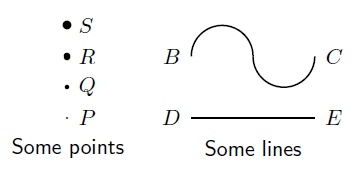
\includegraphics{col11306.imgs/m39370_MG10C13_001.png} % m39370;MG10C13\_001.png;;;6.0;8.5;
      \vspace{2pt}
    \vspace{\rubberspace}\par \begin{cnxcaption}
	  \small \textbf{Figure 12.1: }Examples of some points (labelled $P$, $Q$, $R$ and $S$\hspace{1ex}) and some lines (labelled $BC$ and $DE$\hspace{1ex}).
	\end{cnxcaption}
    \vspace{.1in}
    \rule[.1in]{\figurerulewidth}{.005in} \\
    \end{center}
 \end{figure}       
      \label{m39370*id313170}Lines are labelled according to the start point and end point. We call the line that starts at a point $A$ and ends at a point $B$, $AB$. Since the line from point $B$ to point $A$ is the same as the line from point $A$ to point $B$, we have that $AB=BA$.\par 
      \label{m39370*id313175}When there is no ambiguity (which is the case throughout this text) the length of the line between points $A$ and $B$ is also denoted $AB$\hspace{1ex}, the same as the notation to refer to the line itself. So if we say $AB=CD$\hspace{1ex} we mean that the length of the line between $A$ and $B$ is equal to the length of the line between $C$ and $D$.
\par 
      \label{m39370*eip-313}Note: in higher mathematics, where there might be some ambiguity between when we want refer to the length of the line and when we just want to refer to the line itself, the notation $|AB|$\hspace{1ex} is usually used to refer to the length of the line. In this case, if one says $|AB|=|CD|$, it means the lengths of the lines are the same, whereas if one says $AB=CD$, it means that the two lines actually coincide (i.e. they are the same). Throughout this text, however, this notation will not be used, and $AB=CD$ ALWAYS implies that the lengths are the same. \par \label{m39370*id314000}A line is measured in \textsl{units of length}. Some common units of length are listed in Table 12.1.\par 
    % \textbf{m39370*uid8}\par
          \begin{table}[H]
    % \begin{table}[H]
    % \\ '' '0'
        \begin{center}
      \label{m39370*uid8}
    \noindent
    \tabletail{%
        \hline
        \multicolumn{2}{|p{\mytableboxwidth}|}{\raggedleft \small \sl continued on next page}\\
        \hline
      }
      \tablelasttail{}
      \begin{xtabular}[t]{|l|l|}\hline
                \textbf{Unit of Length}
               &
                \textbf{Abbreviation}
              % make-rowspan-placeholders
     \tabularnewline\cline{1-1}\cline{2-2}
      %--------------------------------------------------------------------
        kilometre &
        km% make-rowspan-placeholders
     \tabularnewline\cline{1-1}\cline{2-2}
      %--------------------------------------------------------------------
        metre &
        m% make-rowspan-placeholders
     \tabularnewline\cline{1-1}\cline{2-2}
      %--------------------------------------------------------------------
        centimetre &
        cm% make-rowspan-placeholders
     \tabularnewline\cline{1-1}\cline{2-2}
      %--------------------------------------------------------------------
        millimetre &
        mm% make-rowspan-placeholders
     \tabularnewline\cline{1-1}\cline{2-2}
      %--------------------------------------------------------------------
    \end{xtabular}
      \end{center}
    \begin{center}{\small\bfseries Table 12.1}: Some common units of length and their abbreviations.\end{center}
    \begin{caption}{\small\bfseries Table 12.1}: Some common units of length and their abbreviations.\end{caption}
\end{table}
    \par
    \label{m39370*cid4}
            \subsection{ Angles}
            \nopagebreak
      \label{m39370*id314141}An \textsl{angle} is formed when two straight lines meet at a point. The point at which two lines meet is known as a \textsl{vertex}. Angles are labelled with a $\phantom{\rule{0.277778em}{0ex}}\hat{}\phantom{\rule{0.277778em}{0ex}}$ called a caret on a letter. For example, in Figure~12.2 the angle is at $\hat{B}$. Angles can also be labelled according to the line segments that make up the angle. For example, in Figure~12.2 the angle is made up when line segments $CB$ and $BA$ meet. So, the angle can be referred to as $\angle CBA$\hspace{1ex} or $\angle ABC$\hspace{1ex} or, if there is no ambiguity (i.e. there is only one angle at $B$) sometimes simply $\angle B$. The $\angle $ symbol is a short method of writing angle in geometry.\par 
      \label{m39370*id314241}Angles are measured in \textsl{degrees} which is denoted by ${}^{\circ }$, a small circle raised above the text in the same fashion as an exponent (or a superscript).\par 
      \label{m39370*eip-522}\label{m39370*notfhsst!!!underscore!!!id43812}
\begin{tabular}{cc}
	\hspace*{-50pt}\raisebox{-8 mm}{\hspace{-0.2in}
\includegraphics[width=0.75in]{col11306.imgs/psfact2.png} } & 
	\begin{minipage}{0.85\textwidth}
	\begin{note}
      {note: }
        \label{m39370*id316245335}Angles can also be measured in radians. At high school level you will only use degrees, but if you decide to take maths at university you will learn about radians.
        \par 
	\end{note}
	\end{minipage}
	\end{tabular}
	\par
      \par 
    \setcounter{subfigure}{0}
	\begin{figure}[H] % horizontal\label{m39370*uid9}
    \begin{center}
    \rule[.1in]{\figurerulewidth}{.005in} \\
        \label{m39370*uid9!!!underscore!!!media}\label{m39370*uid9!!!underscore!!!printimage}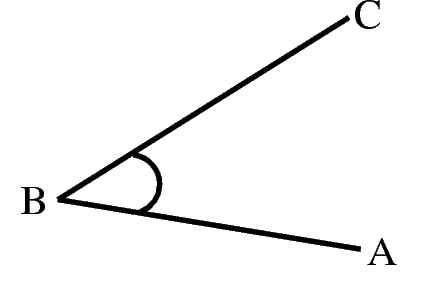
\includegraphics{col11306.imgs/m39370_MG10C13_002.png} % m39370;MG10C13\_002.png;;;6.0;8.5;
      \vspace{2pt}
    \vspace{\rubberspace}\par \begin{cnxcaption}
	  \small \textbf{Figure 12.2: }Angle labelled as $\hat{B}$, $\angle CBA$\hspace{1ex} or $\angle ABC$
	\end{cnxcaption}
    \vspace{.1in}
    \rule[.1in]{\figurerulewidth}{.005in} \\
    \end{center}
 \end{figure}       
    \setcounter{subfigure}{0}
	\begin{figure}[H] % horizontal\label{m39370*uid10}
    \begin{center}
    \rule[.1in]{\figurerulewidth}{.005in} \\
        \label{m39370*uid10!!!underscore!!!media}\label{m39370*uid10!!!underscore!!!printimage}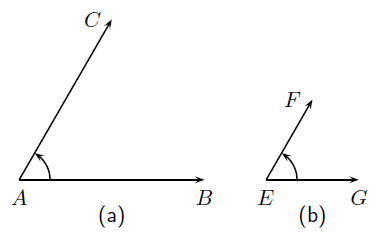
\includegraphics{col11306.imgs/m39370_MG10C13_003.png} % m39370;MG10C13\_003.png;;;6.0;8.5;
      \vspace{2pt}
    \vspace{\rubberspace}\par \begin{cnxcaption}
	  \small \textbf{Figure 12.3: }Examples of angles. $\hat{A}=\hat{E}$, even though the lines making up the angles are of different lengths.
	\end{cnxcaption}
    \vspace{.1in}
    \rule[.1in]{\figurerulewidth}{.005in} \\
    \end{center}
 \end{figure}       
      \label{m39370*uid11}
            \subsubsection{ Measuring angles}
            \nopagebreak
        \label{m39370*id314363}The size of an angle does not depend on the length of the lines that are joined to make up the angle, but depends only on how both the lines are placed as can be seen in Figure~12.3. This means that the idea of length cannot be used to measure angles. An angle is a rotation around the vertex.\par 
        \label{m39370*uid12}
            \subsubsection{ Using a Protractor}
            \nopagebreak
          \label{m39370*id314383}A protractor is a simple tool that is used to measure angles. A picture of a protractor is shown in Figure~12.4.\par 
    \setcounter{subfigure}{0}
	\begin{figure}[H] % horizontal\label{m39370*uid13}
    \begin{center}
    \rule[.1in]{\figurerulewidth}{.005in} \\
        \label{m39370*uid13!!!underscore!!!media}\label{m39370*uid13!!!underscore!!!printimage}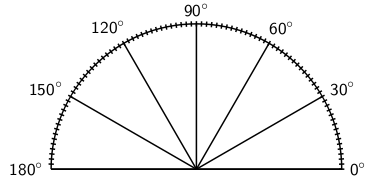
\includegraphics{col11306.imgs/m39370_MG10C13_004.png} % m39370;MG10C13\_004.png;;;6.0;8.5;
      \vspace{2pt}
    \vspace{\rubberspace}\par \begin{cnxcaption}
	  \small \textbf{Figure 12.4: }Diagram of a protractor.
	\end{cnxcaption}
    \vspace{.1in}
    \rule[.1in]{\figurerulewidth}{.005in} \\
    \end{center}
 \end{figure}       
          \label{m39370*id314404}
            \textbf{Method:}
          \par 
          \label{m39370*id314412}Using a protractor\par 
          \label{m39370*id314417}\begin{enumerate}[noitemsep, label=\textbf{\arabic*}. ] 
            \label{m39370*uid14}\item Place the bottom line of the protractor along one line of the angle so that the other line of the angle points at the degree markings.
\label{m39370*uid15}\item Move the protractor along the line so that the centre point on the protractor is at the vertex of the two lines that make up the angle.
\label{m39370*uid16}\item Follow the second line until it meets the marking on the protractor and read off the angle. Make sure you start measuring at 0${}^{\circ }$.
\end{enumerate}
\label{m39370*secfhsst!!!underscore!!!id175}
            \subsubsection{  Measuring Angles : Use a protractor to measure the following angles:}
            \nopagebreak
          \label{m39370*id314481}
    \setcounter{subfigure}{0}
	\begin{figure}[H] % horizontal\label{m39370*id314484}
    \begin{center}
    \label{m39370*id314484!!!underscore!!!media}\label{m39370*id314484!!!underscore!!!printimage}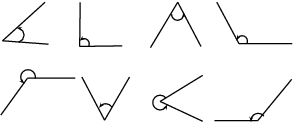
\includegraphics{col11306.imgs/m39370_MG10C13_005.png} % m39370;MG10C13\_005.png;;;6.0;8.5;
      \vspace{2pt}
    \vspace{.1in}
    \end{center}
 \end{figure}       
          \par 
      \label{m39370*uid17}
            \subsubsection{ Special Angles}
            \nopagebreak
        \label{m39370*id314513}What is the smallest angle that can be drawn? The figure below shows two lines ($CA$ and $AB$) making an angle at a common vertex $A$. If line $CA$ is rotated around the common vertex $A$, down towards line $AB$, then the smallest angle that can be drawn occurs when the two lines are pointing in the same direction. This gives an angle of 0${}^{\circ }$. This is shown in Figure~12.6\par 
        \label{m39370*id314590}
    \setcounter{subfigure}{0}
	\begin{figure}[H] % horizontal\label{m39370*id314593}
    \begin{center}
    \label{m39370*id314593!!!underscore!!!media}\label{m39370*id314593!!!underscore!!!printimage}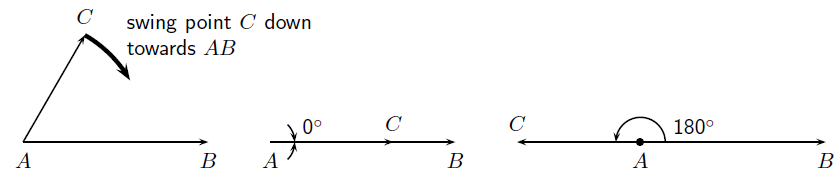
\includegraphics{col11306.imgs/m39370_MG10C13_006.png} % m39370;MG10C13\_006.png;;;6.0;8.5;
      \vspace{2pt}
    \vspace{.1in}
    \end{center}
 \end{figure}       
        \par 
        \label{m39370*id314599}If line $CA$ is now swung upwards, any other angle can be obtained. If line $CA$ and line $AB$ point in opposite directions (the third case in Figure~12.6) then this forms an angle of 180${}^{\circ }$.\par 
\label{m39370*notfhsst!!!underscore!!!id201}
\begin{tabular}{cc}
	   \hspace*{-50pt}\raisebox{-8 mm}{ 
\includegraphics[width=0.5in]{col11306.imgs/pstip2.png}  }& 
	\begin{minipage}{0.85\textwidth}
	\begin{note}
      {tip: }If three points $A$, $B$ and $C$ lie on a straight line, then the angle between them is 180${}^{\circ }$. Conversely, if the angle between three points is 180${}^{\circ }$, then the points lie on a straight line.
	\end{note}
	\end{minipage}
	\end{tabular}
	\par
        \label{m39370*id314704}An angle of 90${}^{\circ }$ is called a \textsl{right angle}. A right angle is half the size of the angle made by a straight line (180${}^{\circ }$). We say $CA$ is \textsl{perpendicular} to $AB$ or $CA\perp AB$\hspace{1ex}. An angle twice the size of a straight line is 360${}^{\circ }$. An angle measuring 360${}^{\circ }$ looks identical to an angle of 0${}^{\circ }$, except for the labelling. We call this a \textsl{revolution}.\par 
    \setcounter{subfigure}{0}
	\begin{figure}[H] % horizontal\label{m39370*uid18}
    \begin{center}
    \rule[.1in]{\figurerulewidth}{.005in} \\
        \label{m39370*uid18!!!underscore!!!media}\label{m39370*uid18!!!underscore!!!printimage}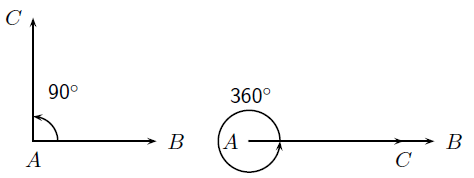
\includegraphics{col11306.imgs/m39370_MG10C13_007.png} % m39370;MG10C13\_007.png;;;6.0;8.5;
      \vspace{2pt}
    \vspace{\rubberspace}\par \begin{cnxcaption}
	  \small \textbf{Figure 12.7: }An angle of 90${}^{\circ }$ is known as a \textsl{right angle}.
	\end{cnxcaption}
    \vspace{.1in}
    \rule[.1in]{\figurerulewidth}{.005in} \\
    \end{center}
 \end{figure}       
\label{m39370*secfhsst!!!underscore!!!id210}
            \subsubsection{  Angles larger than 360${}^{\circ }$ }
            \nopagebreak
        \label{m39370*id314877}All angles larger than 360${}^{\circ }$ also look like we have seen them before. If you are given an angle that is larger than 360${}^{\circ }$, continue subtracting 360${}^{\circ }$ from the angle, until you get an answer that is between 0${}^{\circ }$and 360${}^{\circ }$. Angles that measure more than 360${}^{\circ }$ are largely for mathematical convenience. \par 
\label{m39370*notfhsst!!!underscore!!!id213}
\begin{tabular}{cc}
	   \hspace*{-50pt}\raisebox{-8 mm}{ 
\includegraphics[width=0.5in]{col11306.imgs/pstip2.png}  }& 
	\begin{minipage}{0.85\textwidth}
	\begin{note}
      {tip: }
        \label{m39370*id314971}\begin{itemize}[noitemsep]
            \label{m39370*uid19}\item \textsl{Acute angle}: An angle $\ge {0}^{\circ }$ and $\lessthan{}{90}^{\circ }$.
\label{m39370*uid20}\item \textsl{Right angle}: An angle measuring ${90}^{\circ }$.
\label{m39370*uid21}\item \textsl{Obtuse angle}: An angle $\greatthan{}{90}^{\circ }$ and $\lessthan{}{180}^{\circ }$.
\label{m39370*uid22}\item \textsl{Straight angle}: An angle measuring 180${}^{\circ }$.
\label{m39370*uid23}\item \textsl{Reflex angle}: An angle $\greatthan{}{180}^{\circ }$ and $\lessthan{}{360}^{\circ }$.
\label{m39370*uid24}\item \textsl{Revolution}: An angle measuring ${360}^{\circ }$.
\end{itemize}
        \label{m39370*id315224}These are simply labels for angles in particular ranges, shown in Figure~12.8.\par 
	\end{note}
	\end{minipage}
	\end{tabular}
	\par
    \setcounter{subfigure}{0}
	\begin{figure}[H] % horizontal\label{m39370*uid25}
    \begin{center}
    \rule[.1in]{\figurerulewidth}{.005in} \\
        \label{m39370*uid25!!!underscore!!!media}\label{m39370*uid25!!!underscore!!!printimage}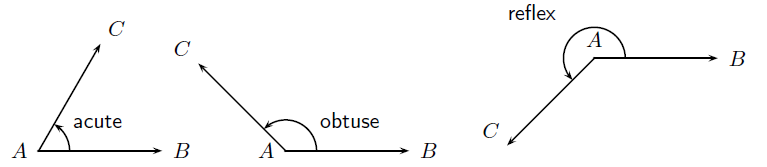
\includegraphics{col11306.imgs/m39370_MG10C13_008.png} % m39370;MG10C13\_008.png;;;6.0;8.5;
      \vspace{2pt}
    \vspace{\rubberspace}\par \begin{cnxcaption}
	  \small \textbf{Figure 12.8: }Three types of angles defined according to their ranges.
	\end{cnxcaption}
    \vspace{.1in}
    \rule[.1in]{\figurerulewidth}{.005in} \\
    \end{center}
 \end{figure}       
        \label{m39370*id315245}Once angles can be measured, they can then be compared. For example, all right angles are 90${}^{\circ }$, therefore all right angles are equal and an obtuse angle will always be larger than an acute angle.\par \label{m39370*eip-752}The following video summarizes what you have learnt so far about angles.
    \setcounter{subfigure}{0}
	\begin{figure}[H] % horizontal\label{m39370*angles-1}
    \textnormal{Khan Academy video on angles - 1}\vspace{.1in} \nopagebreak
  \label{m39370*yt-media1}\label{m39370*yt-video1}
            \raisebox{-5 pt}{ 
\includegraphics[width=0.5cm]{col11306.imgs/summary_www.png}} { (Video:  MG10088 )}
      \vspace{2pt}
    \vspace{.1in}
 \end{figure}       
Note that for high school trigonometry you will be using degrees, not radians as stated in the video. \par 
      \label{m39370*uid26}
            \subsubsection{ Special Angle Pairs}
            \nopagebreak
        \label{m39370*id315274}In Figure~12.10, straight lines $AB$ and $CD$ intersect at point X, forming four angles: $\hat{{X}_{1}}$ or $\angle BXD$\hspace{1ex}, $\hat{{X}_{2}}$\hspace{1ex} or $\angle BXC$\hspace{1ex}, $\hat{{X}_{3}}$\hspace{1ex} or $\angle CXA$\hspace{1ex} and $\hat{{X}_{4}}$\hspace{1ex} or $\angle AXD$\hspace{1ex}.\par 
    \setcounter{subfigure}{0}
	\begin{figure}[H] % horizontal\label{m39370*uid27}
    \begin{center}
    \rule[.1in]{\figurerulewidth}{.005in} \\
        \label{m39370*uid27!!!underscore!!!media}\label{m39370*uid27!!!underscore!!!printimage}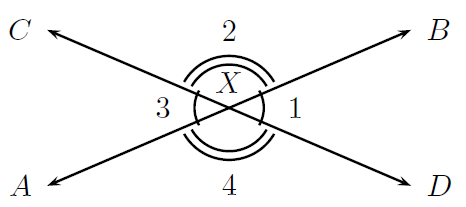
\includegraphics{col11306.imgs/m39370_MG10C13_009.png} % m39370;MG10C13\_009.png;;;6.0;8.5;
      \vspace{2pt}
    \vspace{\rubberspace}\par \begin{cnxcaption}
	  \small \textbf{Figure 12.10: }Two intersecting straight lines with vertical angles $\hat{{X}_{1}},\hat{{X}_{3}}$ and $\hat{{X}_{2}},\hat{{X}_{4}}$.
	\end{cnxcaption}
    \vspace{.1in}
    \rule[.1in]{\figurerulewidth}{.005in} \\
    \end{center}
 \end{figure}       
        \label{m39370*id315545}The table summarises the special angle pairs that result.\par 
    % \textbf{m39370*id315548}\par
          \begin{table}[H]
    % \begin{table}[H]
    % \\ '' '0'
        \begin{center}
      \label{m39370*id315548}
    \noindent
    \tabletail{%
        \hline
        \multicolumn{3}{|p{\mytableboxwidth}|}{\raggedleft \small \sl continued on next page}\\
        \hline
      }
      \tablelasttail{}
      \begin{xtabular}[t]{|l|l|l|}\hline
        Special Angle &
        Property &
        Example% make-rowspan-placeholders
     \tabularnewline\cline{1-1}\cline{2-2}\cline{3-3}
      %--------------------------------------------------------------------
        adjacent angles &
        share a common vertex and a common side &
        $\left(\hat{{X}_{1}},\hat{{X}_{2}}\right)$, $\left(\hat{{X}_{2}},\hat{{X}_{3}}\right)$, $\left(\hat{{X}_{3}},\hat{{X}_{4}}\right)$, $\left(\hat{{X}_{4}},\hat{{X}_{1}}\right)$% make-rowspan-placeholders
     \tabularnewline\cline{1-1}\cline{2-2}\cline{3-3}
      %--------------------------------------------------------------------
        linear pair (adjacent angles on a straight line) &
        adjacent angles formed by two intersecting straight lines that by definition add to 180${}^{\circ }$ &
                  $\hat{{X}_{1}}+\hat{{X}_{2}}={180}^{\circ }$;
                  $\hat{{X}_{2}}+\hat{{X}_{3}}={180}^{\circ }$;
                  $\hat{{X}_{3}}+\hat{{X}_{4}}={180}^{\circ }$;
                  $\hat{{X}_{4}}+\hat{{X}_{1}}={180}^{\circ }$
                % make-rowspan-placeholders
     \tabularnewline\cline{1-1}\cline{2-2}\cline{3-3}
      %--------------------------------------------------------------------
        opposite angles &
        angles formed by two intersecting straight lines that share a vertex but do not share any sides &
                  $\hat{{X}_{1}}=\hat{{X}_{3}}$;
                  $\hat{{X}_{2}}=\hat{{X}_{4}}$
                % make-rowspan-placeholders
     \tabularnewline\cline{1-1}\cline{2-2}\cline{3-3}
      %--------------------------------------------------------------------
        supplementary angles &
      % My position: 1
    % my spanname: 
    % my ct of spanspec: 0
    % my column-count: 2
    \multicolumn{2}{c|}{two angles whose sum is 180${}^{\circ }$}
     \tabularnewline\cline{1-1}\cline{2-2}\cline{3-3}
      %--------------------------------------------------------------------
        complementary angles &
      % My position: 1
    % my spanname: 
    % my ct of spanspec: 0
    % my column-count: 2
    \multicolumn{2}{c|}{two angles whose sum is 90${}^{\circ }$}
     \tabularnewline\cline{1-1}\cline{2-2}\cline{3-3}
      %--------------------------------------------------------------------
    \end{xtabular}
      \end{center}
    \begin{center}{\small\bfseries Table 12.2}\end{center}
    \begin{caption}{\small\bfseries Table 12.2}\end{caption}
\end{table}
    \par
\label{m39370*notfhsst!!!underscore!!!id423}
\begin{tabular}{cc}
	   \hspace*{-50pt}\raisebox{-8 mm}{ 
\includegraphics[width=0.5in]{col11306.imgs/pstip2.png}  }& 
	\begin{minipage}{0.85\textwidth}
	\begin{note}
      {tip: }The opposite angles formed by the intersection of two straight lines are equal. Adjacent angles on a straight line are supplementary.
	\end{note}
	\end{minipage}
	\end{tabular}
	\par
      \label{m39370*eip-433}The following video summarises what you have learnt so far
    \setcounter{subfigure}{0}
	\begin{figure}[H] % horizontal\label{m39370*angles-2}
    \textnormal{Khan Academy video on angles - 2}\vspace{.1in} \nopagebreak
  \label{m39370*yt-media2}\label{m39370*yt-video2}
            \raisebox{-5 pt}{ 
\includegraphics[width=0.5cm]{col11306.imgs/summary_www.png}} { (Video:  MG10089 )}
      \vspace{2pt}
    \vspace{.1in}
 \end{figure}       \par 
      \label{m39370*uid28}
            \subsubsection{ Parallel Lines intersected by Transversal Lines}
            \nopagebreak
            \label{m39370*id316211}Two lines intersect if they cross each other at a point. For example, at a traffic intersection two or more streets intersect; the middle of the intersection is the common point between the streets.\par 
        \label{m39370*id316216}\textsl{Parallel lines} are lines that never intersect. For example the tracks of a railway line are parallel (for convenience, sometimes mathematicians say they intersect at 'a point at infinity', i.e. an infinite distance away). We wouldn't want the tracks to intersect after as that would be catastrophic for the train!\par 
        \label{m39370*id316225}
    \setcounter{subfigure}{0}
	\begin{figure}[H] % horizontal\label{m39370*id316228}
    \begin{center}
    \label{m39370*id316228!!!underscore!!!media}\label{m39370*id316228!!!underscore!!!printimage}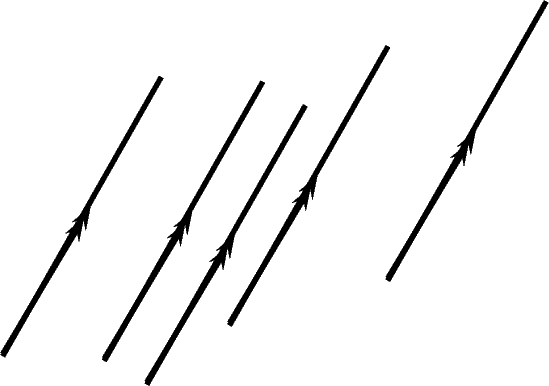
\includegraphics{col11306.imgs/m39370_MG10C13_010.png} % m39370;MG10C13\_010.png;;;6.0;8.5;
      \vspace{2pt}
    \vspace{.1in}
    \end{center}
 \end{figure}       
        \par 
        \label{m39370*id316235}All these lines are parallel to each other. Notice the pair of arrow symbols for parallel.\par 
\label{m39370*notfhsst!!!underscore!!!id438}
\begin{tabular}{cc}
	\hspace*{-50pt}\raisebox{-8 mm}{\hspace{-0.2in}
\includegraphics[width=0.75in]{col11306.imgs/psfact2.png} } & 
	\begin{minipage}{0.85\textwidth}
	\begin{note}
      {note: }
        \label{m39370*id316245}A section of the Australian National Railways Trans-Australian line is perhaps one of the longest pairs of man-made parallel lines.\par 
        \label{m39370*id316258}
          \label{m39370*id316258!!!underscore!!!quote}\begin{quote}{\sl \textbf{Longest Railroad Straight} (Source: www.guinnessworldrecords.com)
The Australian National Railways Trans-Australian line over the Nullarbor Plain, is 478~km (297 miles) dead straight, from Mile 496, between Nurina and Loongana, Western Australia, to Mile 793, between Ooldea and Watson, South Australia.} % end \textsl
    \end{quote}
        \par 
	\end{note}
	\end{minipage}
	\end{tabular}
	\par
        \label{m39370*id316273}A \textsl{transversal} of two or more lines is a line that intersects these lines. For example in Figure~12.13, $AB$ and $CD$ are two parallel lines and $EF$ is a transversal. We say $AB\parallel CD$. The properties of the angles formed by these intersecting lines are summarised in the table below.\par 
    \setcounter{subfigure}{0}
	\begin{figure}[H] % horizontal\label{m39370*uid29}
    \begin{center}
    \rule[.1in]{\figurerulewidth}{.005in} \\
        \label{m39370*uid29!!!underscore!!!media}\label{m39370*uid29!!!underscore!!!printimage}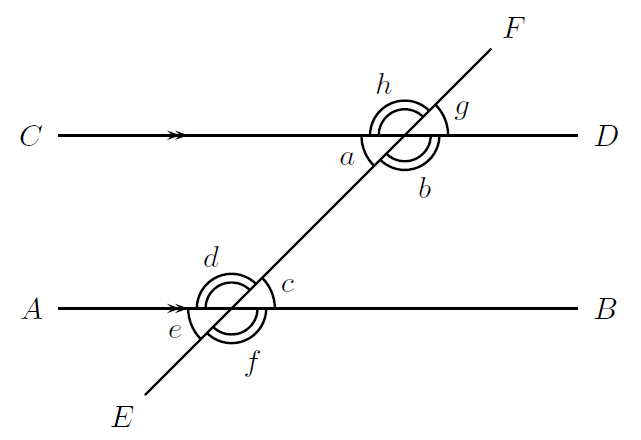
\includegraphics{col11306.imgs/m39370_MG10C13_011.png} % m39370;MG10C13\_011.png;;;6.0;8.5;
      \vspace{2pt}
    \vspace{\rubberspace}\par \begin{cnxcaption}
	  \small \textbf{Figure 12.13: }Parallel lines intersected by a transversal
	\end{cnxcaption}
    \vspace{.1in}
    \rule[.1in]{\figurerulewidth}{.005in} \\
    \end{center}
 \end{figure}       
    % \textbf{m39370*uid30}\par
          \begin{table}[H]
    % \begin{table}[H]
    % \\ '' '0'
        \begin{center}
      \label{m39368*uid92}
    \noindent
    \tabletail{%
        \hline
        \multicolumn{2}{|p{\mytableboxwidth}|}{\raggedleft \small \sl continued on next page}\\
        \hline
      }
      \tablelasttail{}
      \begin{xtabular}[t]{|l|l|}\hline
        Sides &
        Name% make-rowspan-placeholders
     \tabularnewline\cline{1-1}\cline{2-2}
      %--------------------------------------------------------------------
        5 &
        pentagon% make-rowspan-placeholders
     \tabularnewline\cline{1-1}\cline{2-2}
      %--------------------------------------------------------------------
        6 &
        hexagon% make-rowspan-placeholders
     \tabularnewline\cline{1-1}\cline{2-2}
      %--------------------------------------------------------------------
        7 &
        heptagon% make-rowspan-placeholders
     \tabularnewline\cline{1-1}\cline{2-2}
      %--------------------------------------------------------------------
        8 &
        octagon% make-rowspan-placeholders
     \tabularnewline\cline{1-1}\cline{2-2}
      %--------------------------------------------------------------------
        10 &
        decagon% make-rowspan-placeholders
     \tabularnewline\cline{1-1}\cline{2-2}
      %--------------------------------------------------------------------
        15 &
        pentadecagon% make-rowspan-placeholders
     \tabularnewline\cline{1-1}\cline{2-2}
      %--------------------------------------------------------------------
    \end{xtabular}
      \end{center}
    \begin{center}{\small\bfseries Table 12.7}: Table of some polygons and their number of sides.\end{center}
    \begin{caption}{\small\bfseries Table 12.7}: Table of some polygons and their number of sides.\end{caption}
\end{table}
    \par
    \setcounter{subfigure}{0}
	\begin{figure}[H] % horizontal\label{m39368*uid93}
    \begin{center}
    \rule[.1in]{\figurerulewidth}{.005in} \\
        \label{m39368*uid93!!!underscore!!!media}\label{m39368*uid93!!!underscore!!!printimage}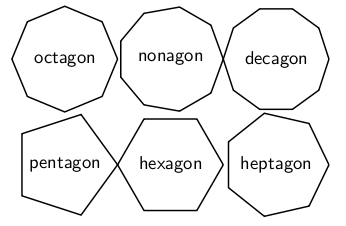
\includegraphics{col11306.imgs/m39368_MG10C13_046.png} % m39368;MG10C13\_046.png;;;6.0;8.5;
      \vspace{2pt}
    \vspace{\rubberspace}\par \begin{cnxcaption}
	  \small \textbf{Figure 12.47: }Examples of other polygons.
	\end{cnxcaption}
    \vspace{.1in}
    \rule[.1in]{\figurerulewidth}{.005in} \\
    \end{center}
 \end{figure}       
      \label{m39368*eip-210}
            \subsubsection{ Angles of Regular Polygons}
            \nopagebreak
            \label{m39368*id319627}Polygons need not have all sides the same. When they do, they are called regular polygons. You can calculate the size of the interior angle of a regular polygon by using:\par 
          \label{m39368*uid96}\nopagebreak\noindent{}
            \settowidth{\mymathboxwidth}{\begin{equation}
    \hat{A}=\frac{n-2}{n}\ensuremath{\times}{180}^{\circ }\tag{12.5}
      \end{equation}
    }
    \typeout{Columnwidth = \the\columnwidth}\typeout{math as usual width = \the\mymathboxwidth}
    \ifthenelse{\lengthtest{\mymathboxwidth < \columnwidth}}{% if the math fits, do it again, for real
    \begin{equation}
    \hat{A}=\frac{n-2}{n}\ensuremath{\times}{180}^{\circ }\tag{12.5}
      \end{equation}
    }{% else, if it doesn't fit
    \setlength{\mymathboxwidth}{\columnwidth}
      \addtolength{\mymathboxwidth}{-48pt}
    \par\vspace{12pt}\noindent\begin{minipage}{\columnwidth}
    \parbox[t]{\mymathboxwidth}{\large$
    \hat{A}=\frac{n-2}{n}\ensuremath{\times}{180}^{\circ }$}\hfill
    \parbox[t]{48pt}{\raggedleft 
    (12.5)}
    \end{minipage}\vspace{12pt}\par
    }% end of conditional for this bit of math
    \typeout{math as usual width = \the\mymathboxwidth}
          \label{m39368*id319678}where $n$ is the number of sides and $\hat{A}$ is any angle.\par \label{m39368*eip-804}\vspace{.5cm} 
      \noindent
      \hspace*{-30pt}
\includegraphics[width=0.5in]{col11306.imgs/pspencil2.png}   \raisebox{25mm}{   
      \begin{mdframed}[linewidth=4, leftmargin=40, rightmargin=40]  
      \begin{exercise}
    \noindent\textbf{Exercise 12.4}\label{m39368*eip-708}
  \label{m39368*eip-618}
    Find the size of the interior angles of a regular octagon.
  \par 
\vspace{5pt}
\label{m39368*eip-937}\noindent\textbf{Solution to Exercise }
\label{m39368*id7432}\begin{enumerate}[noitemsep, label=\textbf{Step} \textbf{\arabic*}. ] 
            \leftskip=20pt\rightskip=\leftskip\item 
An octagon has 8 sides.
\item 
\label{m39368*id7344}\nopagebreak\noindent{}
\settowidth{\mymathboxwidth}{\begin{equation}
    \begin{array}{ccc}\hfill \hat{A}& =& \frac{n-2}{n}\ensuremath{\times}{180}^{\circ }\hfill \\ \hfill \hat{A}& =& \frac{8-2}{8}\ensuremath{\times}{180}^{\circ }\hfill \\ \hfill \hat{A}& =& \frac{6}{2}\ensuremath{\times}{180}^{\circ }\hfill \\ \hfill \hat{A}& =& {135}^{\circ }\hfill \end{array}\tag{12.6}
      \end{equation}
    }
    \typeout{Columnwidth = \the\columnwidth}\typeout{math as usual width = \the\mymathboxwidth}
    \ifthenelse{\lengthtest{\mymathboxwidth < \columnwidth}}{% if the math fits, do it again, for real
    \begin{equation}
    \begin{array}{ccc}\hfill \hat{A}& =& \frac{n-2}{n}\ensuremath{\times}{180}^{\circ }\hfill \\ \hfill \hat{A}& =& \frac{8-2}{8}\ensuremath{\times}{180}^{\circ }\hfill \\ \hfill \hat{A}& =& \frac{6}{2}\ensuremath{\times}{180}^{\circ }\hfill \\ \hfill \hat{A}& =& {135}^{\circ }\hfill \end{array}\tag{12.6}
      \end{equation}
    }{% else, if it doesn't fit
    \setlength{\mymathboxwidth}{\columnwidth}
      \addtolength{\mymathboxwidth}{-48pt}
    \par\vspace{12pt}\noindent\begin{minipage}{\columnwidth}
    \parbox[t]{\mymathboxwidth}{\large$
    \hat{A}=\frac{n-2}{n}\ensuremath{\times}{180}^{\circ }\hat{A}=\frac{8-2}{8}\ensuremath{\times}{180}^{\circ }\hat{A}=\frac{6}{2}\ensuremath{\times}{180}^{\circ }\hat{A}={135}^{\circ }$}\hfill
    \parbox[t]{48pt}{\raggedleft 
    (12.6)}
    \end{minipage}\vspace{12pt}\par
    }% end of conditional for this bit of math
    \typeout{math as usual width = \the\mymathboxwidth}
\end{enumerate}
    \end{exercise}
    \end{mdframed}
    }
    \noindent
    \label{m39368*eip-514}
            \subsection{ Summary}
            \nopagebreak
            \label{m39368*eip-439}\begin{itemize}[noitemsep]
            \item Make sure you know what the following terms mean: quadrilaterals, vertices, sides, angles, parallel lines, perpendicular lines,diagonals, bisectors and transversals.\item The properties of triangles has been covered.\item Congruency and similarity of triangles\item Angles can be classified as acute, right, obtuse, straight, reflex or revolution\item Theorem of Pythagoras which is used to calculate the lengths of sides of a right-angled triangle\item Angles: \label{m39368*id98732}\begin{itemize}[noitemsep]
            \item Acute angle: An angle ${0}^{\circ }$ and ${90}^{\circ }$\item Right angle: An angle measuring ${90}^{\circ }$\item Obtuse angle: An angle ${90}^{\circ }$ and ${180}^{\circ }$\item Straight angle: An angle measuring ${180}^{\circ }$\item Reflex angle: An angle ${180}^{\circ }$ and ${360}^{\circ }$\item Revolution: An angle measuring ${360}^{\circ }$\end{itemize}
        \item There are several properties of angles and some special names for these\item There are four types of triangles: Equilateral, isoceles, right-angled and scalene\item The angles in a triangle add up to ${180}^{\circ }$\end{itemize}
        \label{m39368*cid6}
            \subsection{ Exercises}
            \nopagebreak
            \label{m39368*id320135}\begin{enumerate}[noitemsep, label=\textbf{\arabic*}. ] 
            \label{m39368*uid112}\item Find all the pairs of parallel lines in the following figures, giving reasons in each case.
\label{m39368*eip-78}\begin{enumerate}[noitemsep, label=\textbf{\alph*}. ] 
            \label{m39368*uid113}\item 
    \setcounter{subfigure}{0}
	\begin{figure}[H] % horizontal\label{m39368*id320164}
    \begin{center}
    \label{m39368*id320164!!!underscore!!!media}\label{m39368*id320164!!!underscore!!!printimage}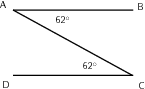
\includegraphics{col11306.imgs/m39368_MG10C13_054.png} % m39368;MG10C13\_054.png;;;6.0;8.5;
      \vspace{2pt}
    \vspace{.1in}
    \end{center}
 \end{figure}       
        \label{m39368*uid114}\item 
    \setcounter{subfigure}{0}
	\begin{figure}[H] % horizontal\label{m39368*id320183}
    \begin{center}
    \label{m39368*id320183!!!underscore!!!media}\label{m39368*id320183!!!underscore!!!printimage}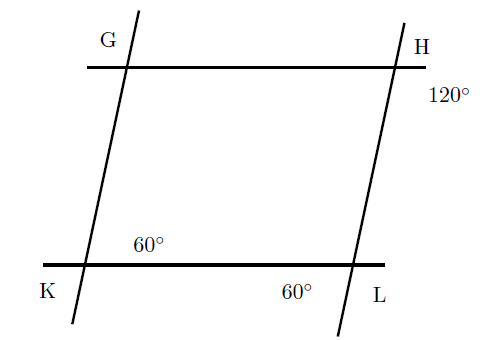
\includegraphics{col11306.imgs/m39368_MG10C13_055.png} % m39368;MG10C13\_055.png;;;6.0;8.5;
      \vspace{2pt}
    \vspace{.1in}
    \end{center}
 \end{figure}       
        \label{m39368*uid115}\item 
    \setcounter{subfigure}{0}
	\begin{figure}[H] % horizontal\label{m39368*id320201}
    \begin{center}
    \label{m39368*id320201!!!underscore!!!media}\label{m39368*id320201!!!underscore!!!printimage}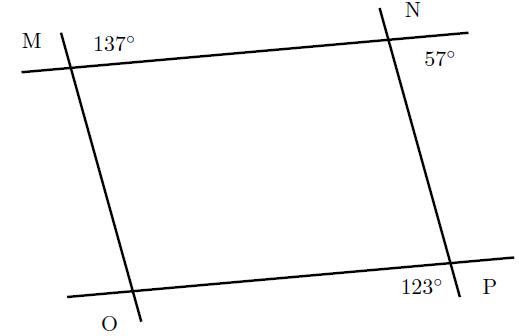
\includegraphics{col11306.imgs/m39368_MG10C13_056.png} % m39368;MG10C13\_056.png;;;6.0;8.5;
      \vspace{2pt}
    \vspace{.1in}
    \end{center}
 \end{figure}       
        \end{enumerate}
        \label{m39368*uid116}\item Find angles $a$, $b$, $c$ and $d$ in each case, giving reasons.
\label{m39368*id320255}\begin{enumerate}[noitemsep, label=\textbf{\alph*}. ] 
            \label{m39368*uid117}\item 
    \setcounter{subfigure}{0}
	\begin{figure}[H] % horizontal\label{m39368*id320271}
    \begin{center}
    \label{m39368*id320271!!!underscore!!!media}\label{m39368*id320271!!!underscore!!!printimage}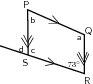
\includegraphics{col11306.imgs/m39368_MG10C13_057.png} % m39368;MG10C13\_057.png;;;6.0;8.5;
      \vspace{2pt}
    \vspace{.1in}
    \end{center}
 \end{figure}       \label{m39368*uid118}\item 
    \setcounter{subfigure}{0}
	\begin{figure}[H] % horizontal\label{m39368*id320290}
    \begin{center}
    \label{m39368*id320290!!!underscore!!!media}\label{m39368*id320290!!!underscore!!!printimage}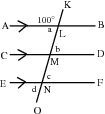
\includegraphics{col11306.imgs/m39368_MG10C13_058.png} % m39368;MG10C13\_058.png;;;6.0;8.5;
      \vspace{2pt}
    \vspace{.1in}
    \end{center}
 \end{figure}       \label{m39368*uid119}\item 
    \setcounter{subfigure}{0}
	\begin{figure}[H] % horizontal\label{m39368*id320310}
    \begin{center}
    \label{m39368*id320310!!!underscore!!!media}\label{m39368*id320310!!!underscore!!!printimage}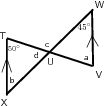
\includegraphics{col11306.imgs/m39368_MG10C13_059.png} % m39368;MG10C13\_059.png;;;6.0;8.5;
      \vspace{2pt}
    \vspace{.1in}
    \end{center}
 \end{figure}       \end{enumerate}
\label{m39368*uid126}\item Say which of the following pairs of triangles are congruent with reasons.
\label{m39368*id320498}\begin{enumerate}[noitemsep, label=\textbf{\alph*}. ] 
            \label{m39368*uid127}\item 
    \setcounter{subfigure}{0}
	\begin{figure}[H] % horizontal\label{m39368*id320512}
    \begin{center}
    \label{m39368*id320512!!!underscore!!!media}\label{m39368*id320512!!!underscore!!!printimage}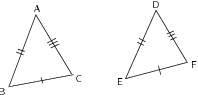
\includegraphics{col11306.imgs/m39368_MG10C13_060.png} % m39368;MG10C13\_060.png;;;6.0;8.5;
      \vspace{2pt}
    \vspace{.1in}
    \end{center}
 \end{figure}       \label{m39368*uid128}\item 
    \setcounter{subfigure}{0}
	\begin{figure}[H] % horizontal\label{m39368*id320530}
    \begin{center}
    \label{m39368*id320530!!!underscore!!!media}\label{m39368*id320530!!!underscore!!!printimage}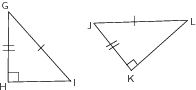
\includegraphics{col11306.imgs/m39368_MG10C13_061.png} % m39368;MG10C13\_061.png;;;6.0;8.5;
      \vspace{2pt}
    \vspace{.1in}
    \end{center}
 \end{figure}       \label{m39368*uid129}\item 
    \setcounter{subfigure}{0}
	\begin{figure}[H] % horizontal\label{m39368*id320548}
    \begin{center}
    \label{m39368*id320548!!!underscore!!!media}\label{m39368*id320548!!!underscore!!!printimage}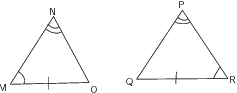
\includegraphics{col11306.imgs/m39368_MG10C13_062.png} % m39368;MG10C13\_062.png;;;6.0;8.5;
      \vspace{2pt}
    \vspace{.1in}
    \end{center}
 \end{figure}       \label{m39368*uid130}\item 
    \setcounter{subfigure}{0}
	\begin{figure}[H] % horizontal\label{m39368*id320565}
    \begin{center}
    \label{m39368*id320565!!!underscore!!!media}\label{m39368*id320565!!!underscore!!!printimage}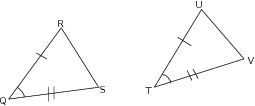
\includegraphics{col11306.imgs/m39368_MG10C13_063.png} % m39368;MG10C13\_063.png;;;6.0;8.5;
      \vspace{2pt}
    \vspace{.1in}
    \end{center}
 \end{figure}       \end{enumerate}
        \label{m39368*uid131}\item Identify the types of angles shown below (e.g. acute/obtuse etc):
    \setcounter{subfigure}{0}
	\begin{figure}[H] % horizontal\label{m39368*id401231}
    \begin{center}
    \label{m39368*id401231!!!underscore!!!media}\label{m39368*id401231!!!underscore!!!printimage}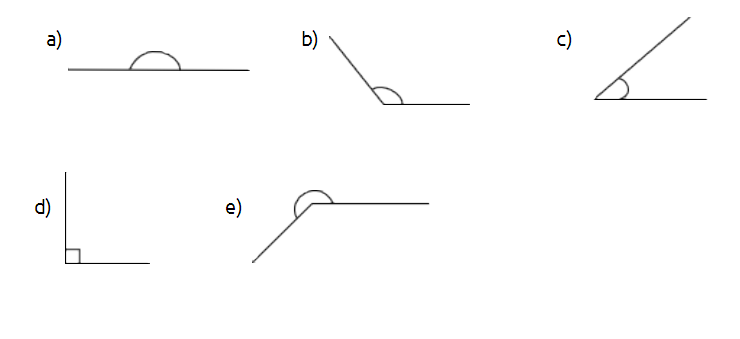
\includegraphics[width=300px]{col11306.imgs/m39368_MG10C13_066.png} % m39368;MG10C13\_066.png;;;6.0;8.5;
      \vspace{2pt}
    \vspace{.1in}
    \end{center}
 \end{figure}       
\label{m39368*uid140}\item Calculate the size of the third angle (x) in each of the diagrams below:
    \setcounter{subfigure}{0}
	\begin{figure}[H] % horizontal\label{m39368*id401232}
    \begin{center}
    \label{m39368*id401232!!!underscore!!!media}\label{m39368*id401232!!!underscore!!!printimage}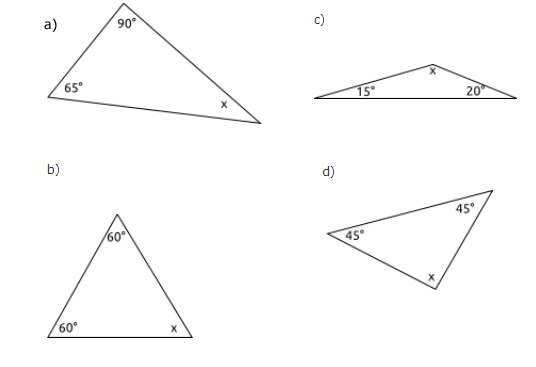
\includegraphics[width=300px]{col11306.imgs/m39368_MG10C13_067.png} % m39368;MG10C13\_067.png;;;6.0;8.5;
      \vspace{2pt}
    \vspace{.1in}
    \end{center}
 \end{figure}       
\label{m39368*uid141}\item Name each of the shapes/polygons, state how many sides each has and whether it is regular (equiangular and equilateral) or not:
    \setcounter{subfigure}{0}
	\begin{figure}[H] % horizontal\label{m39368*id401233}
    \begin{center}
    \label{m39368*id401233!!!underscore!!!media}\label{m39368*id401233!!!underscore!!!printimage}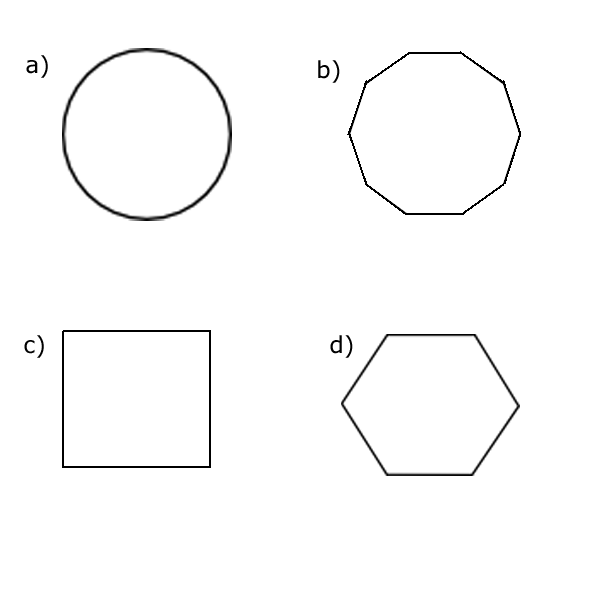
\includegraphics[width=300px]{col11306.imgs/m39368_MG10C13_068.png} % m39368;MG10C13\_068.png;;;6.0;8.5;
      \vspace{2pt}
    \vspace{.1in}
    \end{center}
 \end{figure}       
\label{m39368*uid142}\item Assess whether the following statements are true or false. If the statement is false, explain why:
\label{m39368*id401234}\begin{enumerate}[noitemsep, label=\textbf{\alph*}. ] 
            \item An angle is formed when two straight lines meet at a point.	\item The smallest angle that can be drawn is 5\ensuremath{{\,}^{\circ}}.\item An angle of 90\ensuremath{{\,}^{\circ}} is called a square angle.\item Two angles whose sum is 180\ensuremath{{\,}^{\circ}} are called supplementary angles.\item Two parallel lines will never intersect.\item A regular polygon has equal angles but not equal sides.\item An isoceles triangle has three equal sides.\item If three sides of a triangle are equal in length to the same sides of another triangle, then the two triangles are incongruent.\item If three pairs of corresponding angles in two triangles are equal, then the triangles are similar.\end{enumerate}
\label{m39368*uid143}\item Name the type of angle (e.g. acute/obtuse etc) based on it's size:
\label{m39368*id401235}\begin{enumerate}[noitemsep, label=\textbf{\alph*}. ] 
            \item  30\ensuremath{{\,}^{\circ}}\item  47\ensuremath{{\,}^{\circ}}\item  90\ensuremath{{\,}^{\circ}}\item  91\ensuremath{{\,}^{\circ}}\item  191\ensuremath{{\,}^{\circ}}\item  360\ensuremath{{\,}^{\circ}}\item  180\ensuremath{{\,}^{\circ}}\end{enumerate}
\label{m39368*uid144}\item Using Pythagoras' theorem for right-angled triangles, calculate the length of x:
    \setcounter{subfigure}{0}
	\begin{figure}[H] % horizontal\label{m39368*id401236}
    \begin{center}
    \label{m39368*id401236!!!underscore!!!media}\label{m39368*id401236!!!underscore!!!printimage}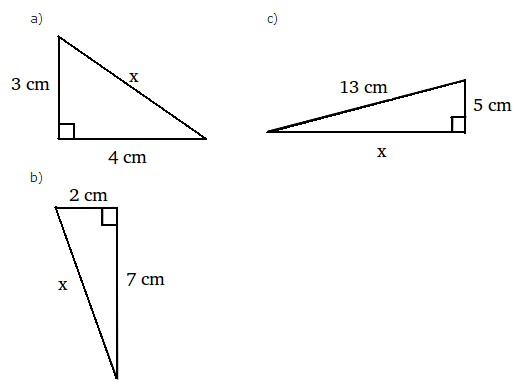
\includegraphics[width=300px]{col11306.imgs/m39368_MG10C13_070.png} % m39368;MG10C13\_070.png;;;6.0;8.5;
      \vspace{2pt}
    \vspace{.1in}
    \end{center}
 \end{figure}       
\end{enumerate}
      \label{m39368*uid132}
\par \raisebox{-0.2em}{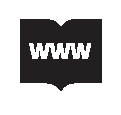
\includegraphics[height=1em]{../icons/www.eps}} Find the answers with the shortcodes:
 \par \begin{tabular}[h]{cccccc}
 (1.) lxh  &  (2.) laq  &  (3.) lai  &  (4.) lTb  &  (5.) lTj  &  (6.) lTD  &  (7.) lTZ  &  (8.) lTB  &  (9.) lTK  & \end{tabular}
            \subsubsection{ Challenge Problem}
            \nopagebreak
        \label{m39368*id320611}\begin{enumerate}[noitemsep, label=\textbf{\arabic*}. ] 
            \label{m39368*uid133}\item Using the figure below, show that the sum of the three angles in a triangle is 180${}^{\circ }$. Line $DE$\hspace{1ex} is parallel to $BC$.
    \setcounter{subfigure}{0}
	\begin{figure}[H] % horizontal\label{m39368*id320668}
    \begin{center}
    \label{m39368*id320668!!!underscore!!!media}\label{m39368*id320668!!!underscore!!!printimage}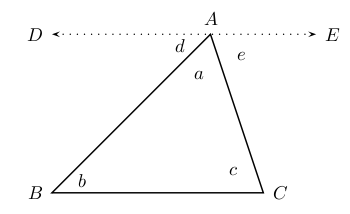
\includegraphics{col11306.imgs/m39368_MG10C13_065.png} % m39368;MG10C13\_065.png;;;6.0;8.5;
      \vspace{2pt}
    \vspace{.1in}
    \end{center}
 \end{figure}       \newline
            \end{enumerate}
  \label{m39368**end}
  \label{8eb3a75df362978731c03bbeab266515**end}
\par \raisebox{-0.2em}{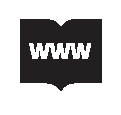
\includegraphics[height=1em]{../icons/www.eps}} Find the answers with the shortcodes:
 \par \begin{tabular}[h]{cccccc}
 (1.) laO  & \end{tabular}
